\section{Design}

\subsection{Data Collection}

The over arching algorithm for collecting data is shown in Figure \ref{fig:main-flow}. For each bus route the following steps occur. \\

\begin{figure}[H]
\begin{center}
    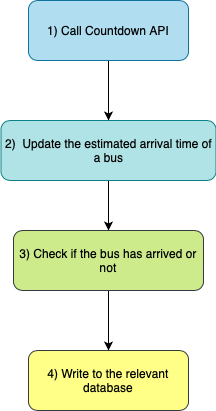
\includegraphics[keepaspectratio, width=5cm]{Images/Data-Collection-new-overarch.png}
    \caption{Overarching data collection algorithm}
    \label{fig:main-flow}
\end{center}
\end{figure}

\textbf{1) Call Countdown API:} Data provided by the Countdown API is stop centric. This means that stop information is crucial to the requests made. Therefore, before the Countdown API can be called, the Stoppoints API must be called to determine the stop ids of all of the stops on a bus route. \\ 

Stoppoints could be called before each Countdown call, however, this is a waste of time since as mentioned in Section \ref{section:tfl-api} Stoppoints returns a mix of valid and invalid stop ids. Therefore, time would have to be spent filtering the Countdown responses to see which have returned expected arrival times and which have returned HTTP errors. Furthermore, it is much faster to access a list of valid stop ids from a database than to retrieve information from an API call. \\

Therefore, it is more computationally efficient to call the Stoppoints API for each bus route used in the data collection process once a week and store the response in a database. Since Countdown only requires the unique national identifier (\texttt{naptanID}) of the bus stop, it is only necessary to extract this parameter from the API response. The common English name of the stop (\texttt{commonName}) is also extracted from the API for ease of data analytics later on. The  \texttt{valid\_stop\_ids\_route} table stores the list of valid stop ids and its respective plain English name for that particular route. A snippet of valid stops for bus route 9 is shown in Figure \ref{fig:valid-stops-db}. The database design is shown in Figure \ref{fig:valid-stops-db-design}. \\

\begin{figure}[H]
\centering
\begin{minipage}{.65\textwidth}
  \centering
  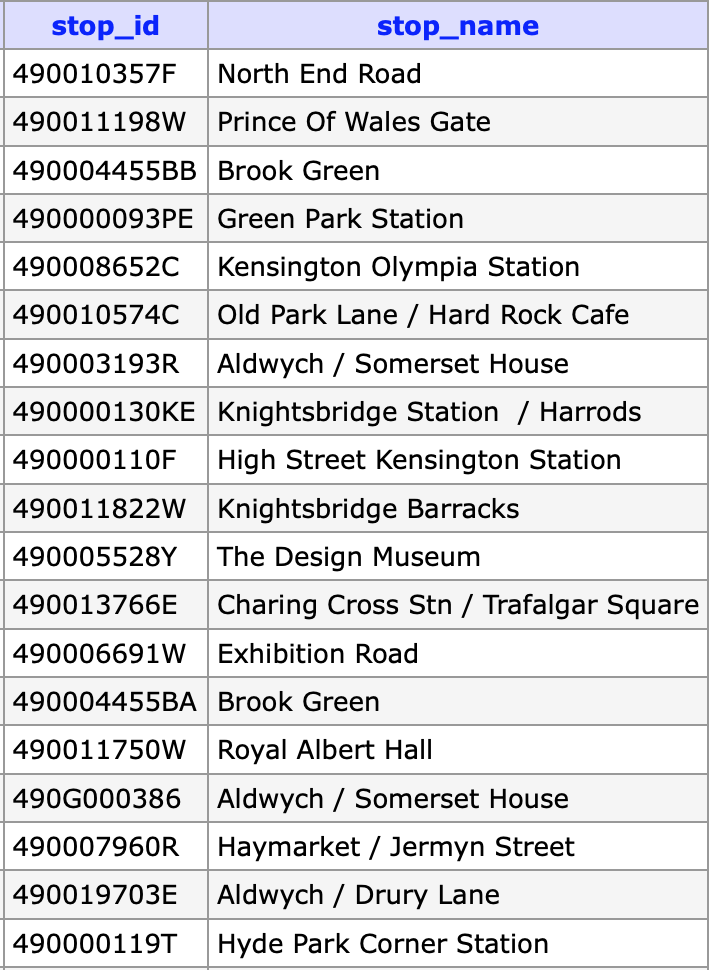
\includegraphics[width=.6\linewidth]{Images/valid-stops.png}
  \caption{Valid Stop Ids Example}
  \label{fig:valid-stops-db}
\end{minipage}%
\begin{minipage}{.35\textwidth}
  \centering
  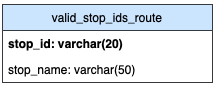
\includegraphics[width=.8\linewidth]{Images/database-diagram-validstops.png}
  \caption{Valid Stop Ids Table}
  \label{fig:valid-stops-db-design}
\end{minipage}
\end{figure}

\textbf{2) Update the estimated arrival time of a bus: } Countdown is called continuously every 30 seconds because as mentioned in Section \ref{section:tfl-api} the information is only updated at source every 30 seconds. If the new expected arrival time returned from the API call is the same as what the database already holds, there is no need to update the item. Otherwise, the database updates both the bus' expected arrival time and the time of the API request. \\

Figure \ref{fig:more-accurate-closer-to-eta} shows two different expected arrival times for Dalgarno Gardens on bus route 7. The figure demonstrates how the predicted arrival time for the same vehicle changes the closer it gets to the actual arrival time. Therefore, data much be collected and updated continuously in order to get as accurate an inferred arrival time as possible.

\begin{figure}[H]
\begin{center}
    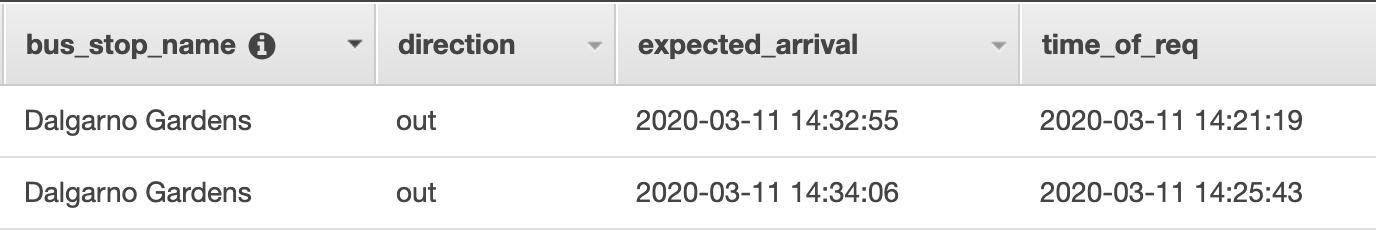
\includegraphics[keepaspectratio, width=15cm]{Images/updated-arrival-time-as-request-is-closer-to-real-time.png}
    \caption{Route 7 data for a particular vehicle X}
    \label{fig:more-accurate-closer-to-eta}
\end{center}
\end{figure}

\textbf{3) Check if the bus has arrived or not: } If a bus \textit{A} is due to arrive at time \textit{X}, when Countdown is called at time \textit{X} and \textit{A} does not appear in the response, it cannot be assumed that \textit{A} has arrived at time \textit{X}. It is possible that there could have been a glitch in the system and \textit{A} has just temporarily vanished. Therefore, the algorithm waits 5 minutes after time \textit{X} and if \textit{A} does not appear in the Countdown response again, then it can be inferred that \textit{A} did indeed arrive at time \textit{X}. However, if during the 5 minutes after time \textit{X} bus  \textit{A} reappears, this implies that \textit{A} will return with a new expected time \textit{Y} and thus did not arrive at time \textit{X}. \\

\textbf{4) Write to the relevant database:} Figure \ref{fig:databases} shows the designs of each of the databases described below.

\begin{itemize}
    \item \texttt{bus\_information\_route} stores information on buses that haven't arrived yet for a particular route.
    \item \texttt{bus\_arrivals\_route} stores information on all buses that have arrived for this route. 
\end{itemize}

\begin{figure}[H]
\begin{center}
    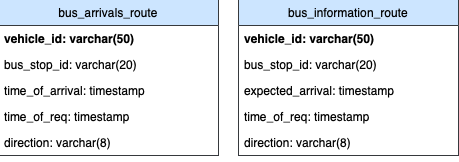
\includegraphics[keepaspectratio, width=12cm]{Images/database-diagrams.png}
    \caption{Databases}
    \label{fig:databases}
\end{center}
\end{figure}

Recall the example Countdown responses in Section \ref{section:tfl-api} for buses arriving at North End Road on bus route 9. Figure \ref{fig:arrived-database} shows how the JSON information has been converted into strings and datetime objects. Specifically, bus \textit{14510} was predicted to arrive at \textit{1589526117000} in UNIX epoch time. This converts to \textit{07:01:57} as seen in the third row of Figure \ref{fig:arrived-database}. The vehicle\_id is a combination of the actual bus id, the stop id, the date of arrival, the direction and the journey number that the bus is on. This is necessary because a particular bus e.g. bus with id \textit{14510} will complete more than one full journey on its route. \\

\begin{figure}[H]
\begin{center}
    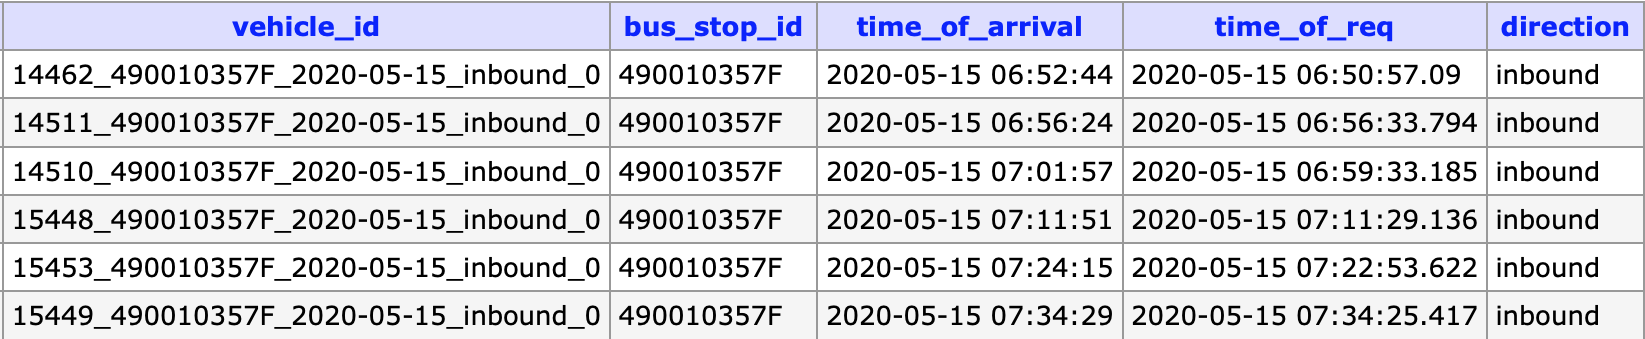
\includegraphics[keepaspectratio, width=16cm]{Images/arrived-northendroad.png}
    \caption{Buses that arrived at North End Road}
    \label{fig:arrived-database}
\end{center}
\end{figure}

\subsubsection{Technology Choices}

This project is quite broad in terms of implementation decisions, therefore, there was no necessity to pick any particular language. Since I had done a lot of projects in Python in my final year of university and because Python has a lot of support online, I chose to write the code that performs the API calls and logic for whether a bus has arrived in Python. \\

Initially, the data collection code was hosted on Amazon Web Services (AWS), using AWS Lambdas to run the data collection functionality and AWS DynamoDB to store the data. AWS Lambda allows code to be run without requiring a server to be provisioned or managed. AWS DynamoDB is a key-value NOSQL database. I chose AWS because its free tier had generous usage and its services worked cohesively together easily and smoothly. Unfortunately, approximately two months into the data collection stage - the code having been left running while I moved on to other parts of the project - I realised that I had exceeded the free tier usage. Therefore, I had to relocate my code onto the DoC Cloud VM.  \\

Paragraph about DoC Cloud VM + docker container. \\

The current data collection code has now changed to use a PostgreSQL database, which is a relational database. This change was done partly because by this point I had already begun writing the code to do the arrival time predictions and I found that it was much more convenient to query for values instead of having to loop through the key value pairs. 

\subsection{Data Exploration}

It is important to explore the dataset collected before building the models in order to understand it better. This could be by discovering patterns, spotting outliers or understanding relationships between variables. TODO CITE \\

For each of the bus routes, graphs were plotted to show the total number of buses arriving at bus stops at different times of day. This helped to see the pattern of numbers of buses according to time of day. For example, from Figure \ref{fig:spread-of-buses-over-day-6} it can be seen that for route 6 during the day, approximately between 0700-1700, there are many more buses on the road, compared to say 2100-0300. 

\begin{figure}[H]
\begin{center}
    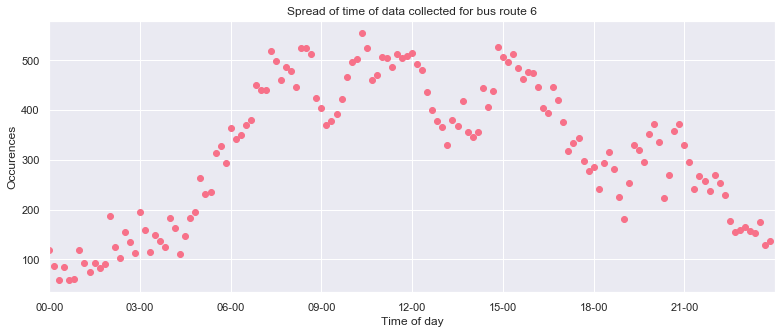
\includegraphics[keepaspectratio, width=15cm]{Images/spread-of-buses-6.png}
    \caption{Number of buses during the day for route 6}
    \label{fig:spread-of-buses-over-day-6}
\end{center}
\end{figure}

Graphs were also plotted to see the total number of buses arriving at bus stops on different days of the week. It was hypothesised that there would be more buses running during weekdays compared to the weekend. However, it can be seen from Figure \ref{fig:spread-of-buses-over-week-6} that there did not seem to be a pattern indicating that the hypothesis was correct.

\begin{figure}[H]
\begin{center}
    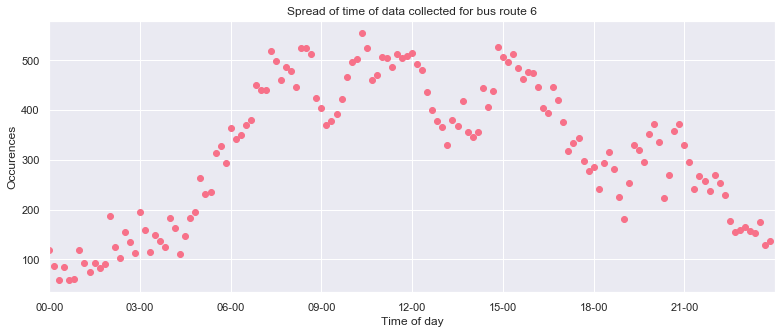
\includegraphics[keepaspectratio, width=15cm]{Images/spread-of-buses-6.png}
    \caption{TODO INSERT FIGURE OF ROUTE 6 DAY OF WEEK SPREAD OF BUSES HERE.}
    \label{fig:spread-of-buses-over-week-6}
\end{center}
\end{figure}

For each route, two bus stops were chosen and the travel times of the bus were calculated. The z-score (Equation \ref{eqn:z-score} was calculated for each journey time and used to measure whether a journey time was an outlier or not. A z-score of larger than 3 or smaller than -3 indicates an outlier TODO CITE. 

\begin{equation}
    z = \frac{x_i - \mu}{\sigma}
    \label{eqn:z-score}
\end{equation}

\noindent Where $x_i$ is a journey time, $\mu$ is the mean and $\sigma$ is the standard deviation. The number of occurrences of a travel time was plotted against the actual travel time, marking the outliers in a different colour. An example of this is seen in Figure \ref{fig:outlier-occurences-52} and Figure \ref{fig:outlier-occurences-9}. Figure \ref{fig:outlier-occurences-52} shows the travel times of bus route 52 between 'All Souls Avenue' and 'Nottinghill Gate Station', whilst Figure \ref{fig:outlier-occurences-9} shows the travel times of bus route 9 between 'North End Road' and 'Phillimore Gardens'. 

\begin{figure}[H]
\begin{center}
    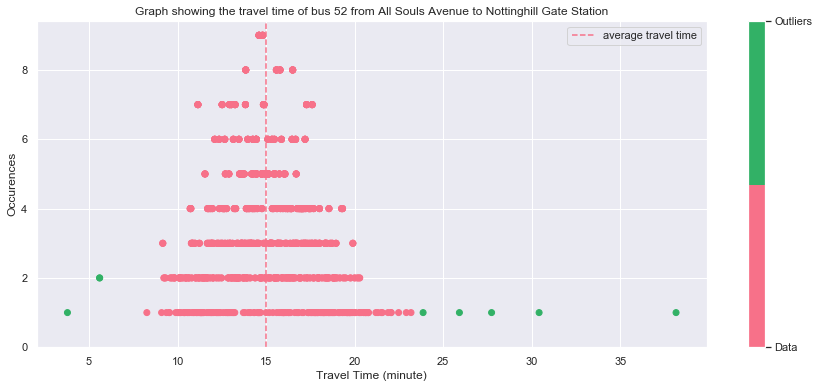
\includegraphics[keepaspectratio, width=15cm]{Images/outliers-52.png}
    \caption{Route 52 travel time and outliers}
    \label{fig:outlier-occurences-52}
\end{center}
\end{figure}

\begin{figure}[H]
\begin{center}
    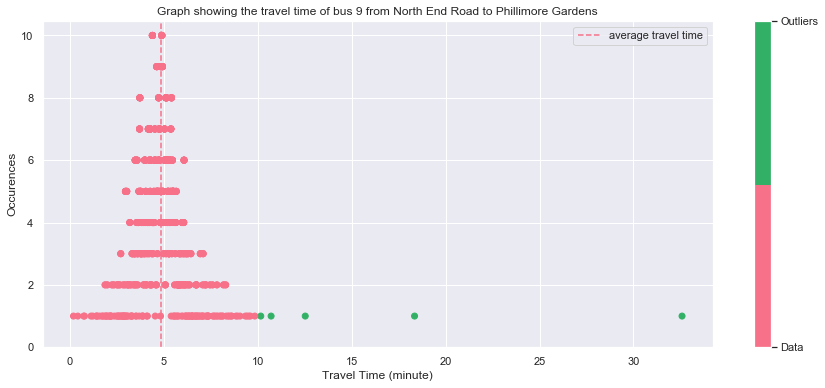
\includegraphics[keepaspectratio, width=15cm]{Images/outliers-9.png}
    \caption{Route 9 travel time and outliers}
    \label{fig:outlier-occurences-9}
\end{center}
\end{figure}

The outliers that have been identified for each route were then removed from the dataset so that the models developed using the data would not be affected by them. \\

The variance and standard deviation were also calculated. For the journey times for buses on route 52 between 'All Souls Avenue' and 'Nottinghill Gate Station', the standard deviation was 2.761 (3sf) and the variance was 7.624 (3sf). For the journey times for buses on route 9 between 'North End Road' and 'Phillimore Gardens', the standard deviation was 1.759 (3sf) and the variance was 3.095 (3sf). 'All Souls Avenue' and 'Nottinghill Gate Station' are 16 stops apart whilst 'North End Road' and 'Phillimore Gardens' are 5 stops apart. Therefore, it was hypothesised that the standard deviation and variance are lower for stops that are closer to each other. In order to confirm this, 'North End Road' was chosen as the start stop and the variance and standard deviation of the journey times between 'North End Road' and stops further away were calculated. The results for between 1 stop away to 16 stops away can be seen in Figure \ref{fig:variance-sd-9}.

\begin{figure}[H]
\begin{center}
    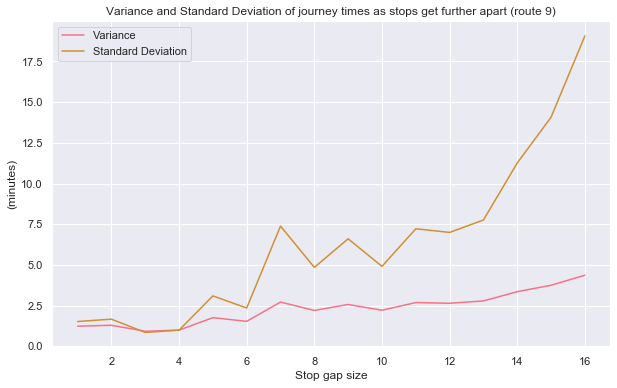
\includegraphics[keepaspectratio, width=15cm]{Images/variance-as-gap-grows.png}
    \caption{Route 9 Variance and Standard Deviation}
    \label{fig:variance-sd-9}
\end{center}
\end{figure}

Based on the results as seen in Figure \ref{fig:variance-sd-9}, it is possible to conclude that there is indeed an upward trend in the variance and standard deviation for stops that are further apart. Therefore, models that use smaller gaps are likely to provide more accurate predictions. This can be seen more obviously in the design of the historical model (Section \ref{section:historical-model-design}). 

\subsubsection{Effect of time of day and time of week}

To see the effect of time of day on bus journey times, the times of day were split into eight sections: 00-03, 03-06, 06-09, 09-12, 12-15, 15-18, 18-21, 21-00. 

For each route two bus stops were chosen and the travel times of the bus were calculated and plotted, as in Figure TODO

\begin{figure}[H]
\begin{center}
    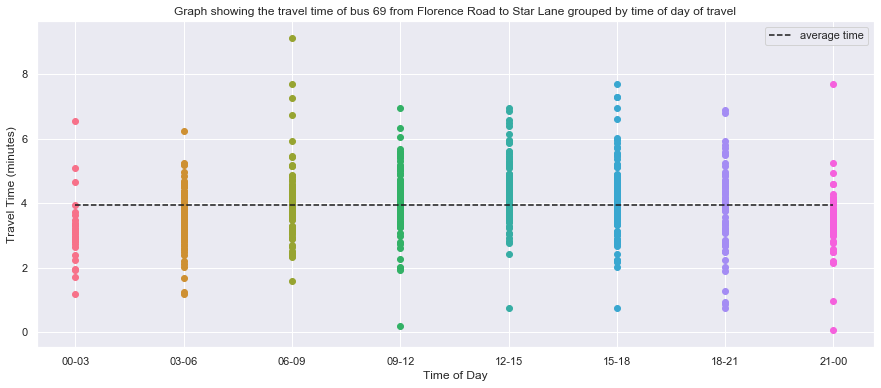
\includegraphics[keepaspectratio, width=15cm]{Images/journey-grouped-by-time-of-day-69.png}
    \caption{Route 52 travel time grouped by time of day}
    \label{fig:time-of-day-52-2}
\end{center}
\end{figure}

\begin{figure}[H]
\begin{center}
    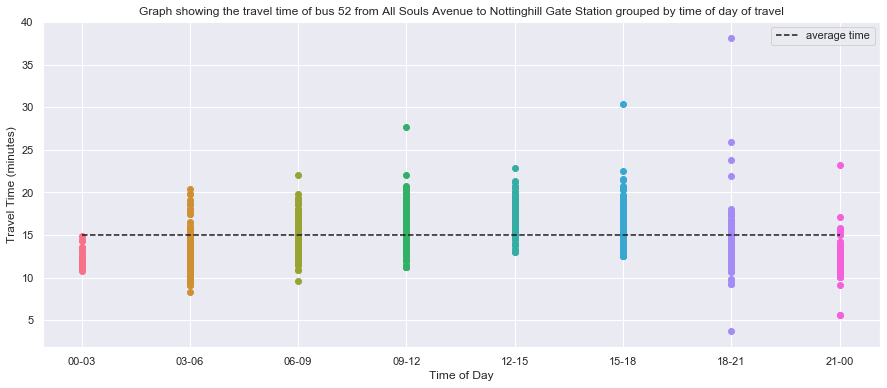
\includegraphics[keepaspectratio, width=15cm]{Images/journey-grouped-by-time-of-day-52.png}
    \caption{Route 69 travel time grouped by time of day}
    \label{fig:time-of-day-69}
\end{center}
\end{figure}

\subsection{Historical Models}
\label{section:historical-model-design}

The historical model is a combination of the mean and naive forecasting methods; it takes the weighted average of the journey times in the past two hours in order to predict the arrival time of a bus for a given stop and route. \\

If the user requests the estimated arrival time of a bus on route X at stop B, the algorithm by which this time is predicted is shown in Figure \ref{fig:historical-flow}: 

\begin{figure}[H]
\begin{center}
    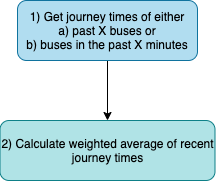
\includegraphics[keepaspectratio, width=5cm]{Images/Historical-Model-overarch.png}
    \caption{Overarching historical model}
    \label{fig:historical-flow}
\end{center}
\end{figure}

\textbf{1) Look for the leave stop}: For route X, find what stop is 5 stops before stop B. Denote this stop as stop A, which will be used to calculate the journey time of the buses. For the first five stops, use the origin stop as stop A. \\

In some cases buses run very infrequently. For example in the early morning hours (0200 - 0400) for bus routes 52 or 69, the buses are timetabled to come every thirty minutes or on special holidays, buses may only run once an hour. Since Countdown only gives information for buses in the next thirty minutes, this means that looking back 5 stops is sometimes insufficient. Consider the following example: a bus arrival time is requested at 0345 at stop 'Star Lane' for route 69. The algorithm looks back 5 stops to get stop 'Florence Road'. However, according to the historical data collected, there is no bus that arrived at 'Florence Road' recently. This could be because the nearest bus is more than thirty minutes away from 'Florence Road'. In cases like this, it is necessary to look back further than 5 stops in order to find the nearest bus on the route. Therefore, the algorithm looks back further until it either reaches a stop which has a bus that has arrived or reaches the origin stop of the route. This becomes the new stop A. The two possible cases are shown in Figures \ref{fig:bigger-gap-a} and \ref{fig:bigger-gap-b}. Figure \ref{fig:bigger-gap-a} shows the case where the algorithm looks back until it reaches a stop where a bus has arrived and Figure \ref{fig:bigger-gap-b} shows the case where the algorithm looks back until it reaches the origin stop. 

\begin{figure}[H]
\begin{center}
    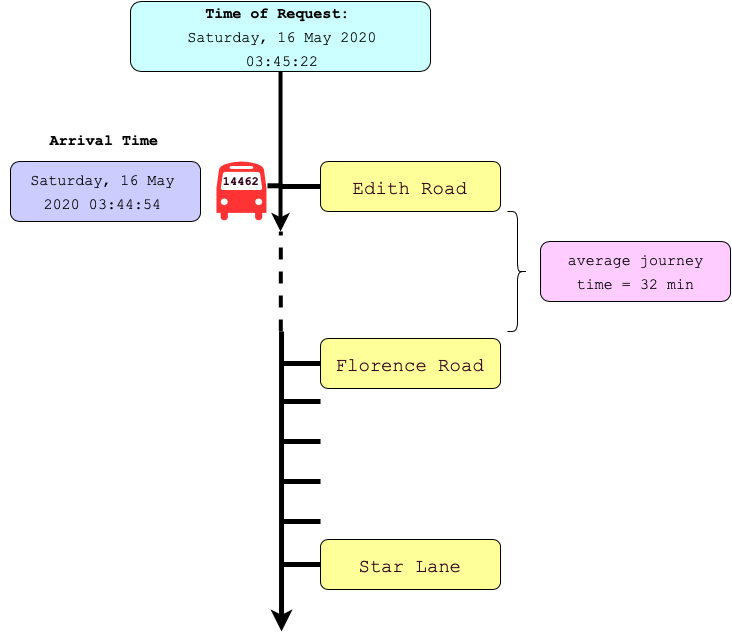
\includegraphics[keepaspectratio, width=10cm]{Images/historical-gap-b.png}
    \caption{Stop A = Edith Road}
    \label{fig:bigger-gap-a}
\end{center}
\end{figure}

\begin{figure}[H]
\begin{center}
    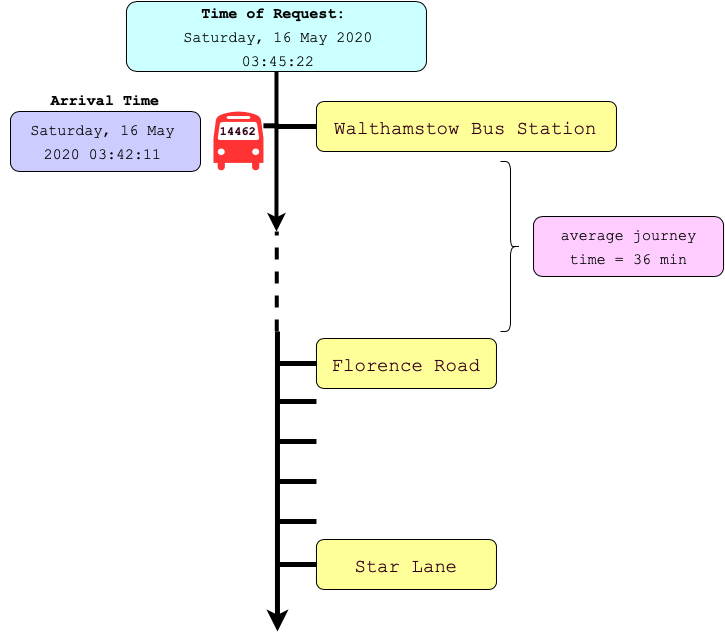
\includegraphics[keepaspectratio, width=10cm]{Images/historical-gap-a.png}
    \caption{Stop A = Walthamstow Bus Station}
    \label{fig:bigger-gap-b}
\end{center}
\end{figure}

Therefore, it can be seen that gaps of larger than 5 will occasionally come into use. Gaps of between 5 to 30 were tried for the same route. It was found that when using stops that were further away from each other, the explained variance score for the predicted arrival times was lower than for stops that were closer together. This implies that using larger gaps between stops provides less accurate predicted arrival times. \\

TODO INSERT EXPLAINED VARIANCE SCORES \\

\textbf{2) Calculate the predicted journey time}: First calculate all the journey times in the past two hours between these two stops. A journey counts if it arrived at stop B both before the request time and within the past two hours. Then, calculate the weighted average to form the predicted journey time for a bus from stop A to stop B. \\

The weights have been chosen so that the buses that arrived at the stop B in the past 10 minutes take priority over the buses that arrived in the past 20 minutes. The buses that arrived in the past 20 minutes have a higher weight than buses that arrived in the past 40 minutes and so on for all the buses in the past two hours. The full weightings is as below:

\begin{multicols}{2}
\begin{itemize}
    \item up to 10 minutes = 0.6
    \item up to 20 minutes = 0.25
    \item up to 40 minutes = 0.1
    \item up to 80 minutes = 0.04
    \item up to 120 minutes = 0.01
\end{itemize}
\end{multicols}

\textbf{3) Find the nearest bus to arrive on or after the request time}: Look through the historical data collected to find the first bus to leave stop A before the request time, but has yet to arrive at stop B. This bus will not be part of the list of buses used to calculated the predicted journey time because it has yet to arrive at stop B. Add the predicted journey time plus thirty seconds to the time this bus leaves stop A to get the predicted arrival time at stop B. The thirty seconds is used as leeway for loading and unloading passengers at a bus stop. \\

If no such bus is found, this indicates that there are no buses currently running this route at the time of request. However, this should be very rare, for example if there is only one bus running the entire route. In these cases, the predicted arrival time will be based purely on historical data, without taking into account recent data (as there is no recent data to take into account). 

\subsubsection{Evaluating the model}

The bus that was used to calculate the predicted arrival time has a vehicle id that is used to find its actual arrival time. The explained variance score of the predicted and actual arrival time is calculated to evaluate the quality of the estimated arrival time. 

\subsubsection{Technology Choices}

Python, Jupyter Notebook, sklearn

\subsection{Regression Models}

Takes into account time of day for a multilinear regression model maybe? 

\clearpage